\chapter{Utility Classes}

Next to the main modules described in the previous chapter, {\tt libbats} offers a collection of utility classes. We will discuss these here.

\lstset{numbers=none}

\section{Rf}
\label{secRf}

When working with pointers and dynamic memory allocation, things could get messy. A memory leak is easily produced and premature deletion of data can cause crashes. The {\tt libbats} library uses a garbage collection system to handle these problems, in the form of the {\tt rf<T>} template class. This class is a wrapper around a pointer, keeps track of the number of times the pointer is used and deletes the data when this number is zero (i.e. it performs reference counting). Its behavior is similar to the smart pointers offered by the Boost library. An {\tt rf} is mostly interchangeable with regular pointers; all operations you usually do directly on a pointer you can do on an {\tt rf} and one can be assigned to the other:
\begin{lstlisting}[frame=single]
rf<MyClass> myRf = new MyClass();
myRf->doSomething();
MyClass& myReference = *myRf;
\end{lstlisting}

It is recommended to use {\tt rf}'s any time you want to use dynamically allocated memory. When you create your own class that you want to be used with {\tt rf}, it is required that that class extends the {\tt RefAble} class. This is needed for the reference counting to work:
\begin{lstlisting}[frame=single]
#include <bats/RefAble/refable.hh>
class MyClass : public bats::RefAble
{
  // Member definitions
};
\end{lstlisting}

\section{Singleton}
\label{secSingleton}

Many modules of the library are so called singletons, so we will give a short introduction about what this is and how they are used. The singleton pattern is a design pattern that makes sure that there is no more than one instance of a certain class. For instance, there is only one Queen of The Netherlands, it would make no sense to create multiple instances. In the singleton design pattern, special measures are taken to prevent you from copying the single instance or creating new objects of the class. This pattern is used in the library for modules for which it makes no sense and for which it could cause problems if there are multiple instances. This is for instance the case for modules keeping track of states, such as the {\tt Localizer} and the {\tt AgentModel}, and a module for maintaining the connection with the server.

In this library, singletons are implemented by the {\tt Singleton<T>} template class. It offers the static {\tt getInstance()} method to request a reference to the single instance of class {\tt T}. For instance, the following shows how to get a reference to the {\tt WorldModel}:
\begin{lstlisting}[frame=single]
WorldModel& wm = Singleton<WorldModel>::getInstance();
\end{lstlisting}
For each singleton class of the library, a {\tt typedef} is set for the {\tt Singleton<T>} instantiation of that class, formed by prefixing the class name with a capital S. So another way to write the previous example would be:
\begin{lstlisting}[frame=single]
WorldModel& wm = SWorldModel::getInstance();
\end{lstlisting}

If you want to use the {\tt Singleton<T>} template to create singletons of your own classes, make sure it adhears to the following points:
\begin{itemize}
\item Your class must have a default constructor.
\item Make all constructors, including the copy constructor, of your class private. 
\item Make the assign operator, {\tt operator=}, private.
\item Define {\tt Singleton<T>}, instantiated with your own class, as friend of your class.
\end{itemize}
If you do this, your class definition will look like this:
%\lstset{numbers=left,numberstyle=\small}
\begin{lstlisting}[frame=single]
class MySingleton
{
  friend class bats::Singleton<MySingleton>;
private:
  // Default constructor
  MySingleton() {}
  // Copy constructor, not implemented
  MySingleton{MySingleton const& other);
  // Assignment operator, not implemented
  MySingleton& operator=(MySingleton const& other);
public:
  // Some public stuff
};
// libbats style singleton typedef
typedef bats::Singleton<MySingleton> SMySingleton;
\end{lstlisting}

\section{Distribution}

Agents often have to work with uncertainty and probability distributions. For instance, vision data received from the simulator is limited and noisy, therefore location estimates derived from this data are just that: estimates, with a certain variability. To deal with this, {\tt libbats} offers the {\tt Distribution} template. This template supports distributions over any number of dimensions, though most commonly 1D distributions, e.g. for joint angles, and 3D distributions, e.g. for locations, are used. Currently there is only a single implementation of this template, the {\tt NormalDistribution}, however it is possible to create new distribution types, like Monte Carlo or histogram based representations.

The most common operation on a distribution is to get the mean value, or 'the most likely' value, which is done with the {\tt getMu()} method. For instance, when asking the {\tt Localizer} for a location, it returns a ({\tt rf} to a) 3D distribution, so to get the most likely local location of the ball you use:
%\lstset{numbers=left,numberstyle=\small}
\begin{lstlisting}[frame=single]
Vector3D ballLoc = localizer.getLocationLocal(Types::BALL)->getMu();
\end{lstlisting}

Other useful methods are {\tt getSigma()}, to get the distribution's covariance matrix, and {\tt draw()}, to draw a random value from the distribution:
%\lstset{numbers=left,numberstyle=\small}
\begin{lstlisting}[frame=single]
Matrix3d ballVariance = localizer.getLocationLocal(Types::BALL)->getSigma();
// 1 dimensional normal distribution
rf<Distribution> myDist = new NormalDistribution(1)
// Initialize distribution with mean 0 and variance 1
Vector1d mu = Vector1d::Zero();
Matrix1d sigma = Matrix1d::Ones();
myDist->init(mu, sigma);
// Draw a random value
Vector3d v = myDist->draw();
\end{lstlisting}

\section{Math}
Several common mathematical problems that are useful in 3D Soccer Simulation are included in {\tt libbats} as methods of the {\tt Math} class. Some of these are pretty selfexplenatory, for the rest see the following descriptions (and again the documentation in the code itself):

\begin{tabular}{l l}
\begin{minipage}{0.7\textwidth}
\begin{description}
\item[distanceLinePoint] This method is used to calculate the distance between a line and a point. The line, dashed black in the example to the right, is defined by a point vector $l_0$ and a direction vector $\vec{l}$, the point $p$ is also a point vector. The method returns the length of the red, dashed line $d$.
\end{description}
\end{minipage}
&
\begin{minipage}{0.3\textwidth}
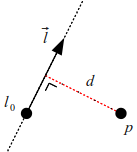
\includegraphics[width=2.5cm]{distlp.png}
\end{minipage}
\end{tabular}

\begin{tabular}{l l}
\begin{minipage}{0.7\textwidth}
\begin{description}
\item[linePointClosestToPoint] This method is used to determine the point on a line that is closest to a given point. The line, dashed black in the example to the right, is defined by a point vector $l_0$ and a direction vector $\vec{l}$, the point $p_0$ is also a point vector. The method returns the coordinates of point $p_1$.
\end{description}
\end{minipage}
&
\begin{minipage}{0.3\textwidth}
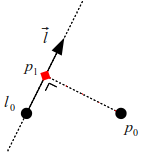
\includegraphics[width=2.5cm]{pointlcp.png}
\end{minipage}
\end{tabular}

\begin{tabular}{l l}
\begin{minipage}{0.7\textwidth}
\begin{description}
\item[intersectVectorPlane] Determine the coordinates of the intersection of a line with a plane. The line, dashed black in the example to the right, is defined by a point vector $l_0$ and a direction vector $\vec{l}$. The plane is defined by the vector $(a, b, c, d)^T$, such that $ax + by + cz = d$. In this representation, the vector $(a,b,c)^T$ is normal to the plane and $d$ is the distance of the plane to the origin of the reference frame. The method returns the coordinates of point $p$.
\end{description}
\end{minipage}
&
\begin{minipage}{0.3\textwidth}
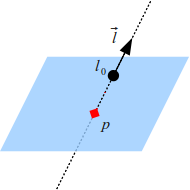
\includegraphics[width=3cm]{intersectvectorplane.png}
\end{minipage}
\end{tabular}

\section{Conf}

\lstset{numbers=left,numberstyle=\scriptsize}

The {\tt libbats} library includes an XML based configuration module, realized by the {\tt Conf} class. This module is for instance used by the {\tt AgentModel} to load the specifications of the robot model, such as sizes, weights and joint names. It is also possible to add new configuration settings, which you can use in your own code.

As most modules, {\tt Conf} is a singleton. When a reference to it is requested for the first time, it loads the default configuration file {\tt conf.xml}, which is supplied and installed allong with the library (it can be found in the {\tt xml} directory and is usually installed in {\tt /usr/local/share/libbats/}). Listing~\ref{codeConfXml} shows the content of this file.

\begin{lstlisting}[float=b,caption={\tt conf.xml},label=codeConfXml,frame=single]
<?xml version="1.0" encoding="ISO-8859-1"?>
<conf xmlns:xi="http://www.w3.org/2003/XInclude">  
  <player-class id="nao">
    <xi:include href="nao_mdl.xml"/>
  </player-class>

  <player id="0" class="nao" />
  <player id="1" class="nao" />
  <player id="2" class="nao" />
  <player id="3" class="nao" />
  <player id="4" class="nao" />
  <player id="5" class="nao" />
  <player id="6" class="nao" />
  <player id="7" class="nao" />
  <player id="8" class="nao" />
  <player id="9" class="nao" />
  <player id="10" class="nao" />
  <player id="11" class="nao" />
</conf>    
\end{lstlisting}

The configuration file has to contain at least the following elements:
\begin{description}
\item[Root] The root node should be a {\tt conf} element. (lines 2 and 19)
\item[Player definition] For each uniform number used, a {\tt player} element should be added. These elements should have an {\tt id} attribute, which is the uniform number, and a {\tt class} attribute, which determines of which class a player is. (lines 7-18)
\item[Classes] Each player can be of a different class, e.g. keeper, defender or attacker, and each class can have different configuration settings. To achieve this, a {\tt player-class} element should be added for each class, with an appropriate {\tt id} attribute. A player class is given to a player by setting its {\tt id} as value of the player's {\tt class} attribute. (lines 3 and 5)
\item[Model] For each player class a model description should be given. The description for the Nao-based model used in the 3D Soccer Simulation competitions is supplied with the library in the file {\tt nao\_mdl.xml} and included in the default configuration. There is most likely no need for you to change this. (line 4)
\end{description}

\lstset{numbers=none}

Besides these necessary elements, there are a few optional configuration settings used by the library. Currently these only include field dimensions (length, width and goal width), and a setting whether or not a match is restarted and the teams switch sides at half-time, which is used to determine who gets the kick-off in the second half. These setting are global and the same for all players, so they are placed in a {\tt parameters} element directly under the root node:
\begin{lstlisting}[frame=single,language=xml]
<conf xmlns:xi="http://www.w3.org/2003/XInclude">
  <parameters>
    <fieldlength>18</fieldlength>
    <fieldwidth>12</fieldwidth>
    <goalwidth>2.1</goalwidth>
    <halftimerestart>1</halftimerestart> <!-- 1 = true, 0 = false -->
  </parameters>
  
  ...
\end{lstlisting}
If these parameters are missing, default values will be loaded (which are the values shown above).

It is easy to create your own configuration file. Just make a copy of the default XML file and make sure that this file is loaded by {\tt Conf} at the beginning of execution:
\begin{lstlisting}[frame=single]
Conf& conf = SConf::getInstance();
conf.setFile("myconf.xml");
\end{lstlisting}
The parameter given to {\tt setFile} should be the path to your configuration file, relative to your agent's binary.

You can now add new parameters to the global {\tt parameters} element, the value of which can be retrieved at runtime using {\tt Conf}'s {\tt getParam} method. This method requires a default value, to be able to determine the type of the parameter, and which is used when the parameter is not defined in the configuration file:
\begin{lstlisting}[frame=single]
// Get the value of the formation parameter.
// e.g. <formation>2</formation>.
// This parameter should be defined in the configuration file,
// If it is not defined, the default value (here 1) will be used
int formation = conf.getParam("formation", 1);
\end{lstlisting}

It is also possible to set parameters specific to a player class. To do so, include a {\tt parameters} element into the appropriate {\tt player-class} element, having the same form a the global version. The value of a parameter for a certain player class can now retrieved by passing the class's id along to {\tt getParam}. The id of the player class of the current agent can be retrieved from the {\tt AgentModel}:
\begin{lstlisting}[frame=single]
// am is a reference to the AgentModel instance
int myformation = conf.getParam(am.getPlayerClass(), "formation", 1);
\end{lstlisting}

These methods are sufficient to set up a basic configuration. For more complex configuration, {\tt Conf} offers the {\tt selectXPath} method, with which you can select any part of the XML file using X-Path queries\footnote{See \url{http://www.w3.org/TR/xpath/} and \url{http://www.w3schools.com/xpath/}}. This allows you to make your configuration as extensive as you want:
\begin{lstlisting}[frame=single]
// Find out the unum of the team captain
string xpath = "/conf/player[class=/conf/player-class/parameters[captain=1]/../@id]/@id";
int unum = conf.selectXPath(xpath).front().getContent().c_str().atoi();
\end{lstlisting}

\section{Types}

The {\tt Types} class holds many useful types and enumerations, used throughout the library. Here is a brief overview of these, but also make sure to look at the code documentation.
\begin{description}
\item[PlayMode] This enumeration list all the possible play modes. For modes of which there are two side variants, e.g. kick-off and free kick, there is also an 'us' and a 'them' version. It is recommended to use these instead of the left/right versions, and all {\tt libbats} modules use the us/them versions. For instance, if the left team gets the kick-off, and our team plays on the right, {\tt WorldModel::getPlayMode()} will return {\tt Types::KICKOFF\_THEM}.
\item[Side] A simple enumeration to discern left and right in a human-readable manner.
\item[Joint] An enumeration of all the agent's joints. This is for instance used to get the current angle of a joint from the {\tt AgentModel}:
\begin{lstlisting}[frame=single]
// Get angle of the first joint of the left arm, in radians
double angle = am.getJoint(Types::LARM1)->angle.getMu()(0);
\end{lstlisting}
\item[BodyPart] An enumeration of all the agent's body parts. This is for instance used to get the current location of a body part from the {\tt AgentModel}:
\begin{lstlisting}[frame=single]
// Get the position of the left foot, relative to the torso
Vector3d pos = am.getBodyPart(Types::LFOOT)->transform.translation;
\end{lstlisting}
\item[Object] This enumeration lists all objects in the environment, such as the ball, players, opponents, and landmarks. For the latter there are left/right and us/them versions. Again, it is recommended to use the us/them variants:
\begin{lstlisting}[frame=single]
// Get the location of the first post of the opponent goal,
// in local coordinates
Vector3d pos = localizer.getLocaltionLocal(Types::GOAL1THEM)->getMu();
\end{lstlisting}
\end{description}

